\documentclass[journal,12pt,twocolumn]{IEEEtran}
\usepackage{setspace}
\usepackage{gensymb}
\singlespacing
\usepackage[cmex10]{amsmath}
\usepackage{amsthm}
\usepackage{mathrsfs}
\usepackage{txfonts}
\usepackage{stfloats}
\usepackage{bm}
\usepackage{cite}
\usepackage{cases}
\usepackage{subfig}
\usepackage{longtable}
\usepackage{multirow}
\usepackage{enumitem}
\usepackage{mathtools}
\usepackage{steinmetz}
\usepackage{tikz}
\usepackage{circuitikz}
\usepackage{verbatim}
\usepackage{tfrupee}
\usepackage[breaklinks=true]{hyperref}
\usepackage{graphicx}
\usepackage{tkz-euclide}
\usetikzlibrary{calc,math}
\usepackage{listings}
\usepackage{color}                                            %%
\usepackage{array}                                            %%
\usepackage{longtable}                                        %%
\usepackage{calc}                                             %%
\usepackage{multirow}                                         %%
\usepackage{hhline}                                           %%
\usepackage{ifthen}                                           %%
\usepackage{lscape}     
\usepackage{multicol}
\usepackage{chngcntr}
\DeclareMathOperator*{\Res}{Res}
\renewcommand\thesection{\arabic{section}}
\renewcommand\thesubsection{\thesection.\arabic{subsection}}
\renewcommand\thesubsubsection{\thesubsection.\arabic{subsubsection}}
\renewcommand\thesectiondis{\arabic{section}}
\renewcommand\thesubsectiondis{\thesectiondis.\arabic{subsection}}
\renewcommand\thesubsubsectiondis{\thesubsectiondis.\arabic{subsubsection}}
\hyphenation{op-tical net-works semi-conduc-tor}
\def\inputGnumericTable{}                                 %%
\lstset
{
%language=C,
frame=single, 
breaklines=true,
columns=fullflexible
}
\begin{document}
\newtheorem{theorem}{Theorem}[section]
\newtheorem{problem}{Problem}
\newtheorem{proposition}{Proposition}[section]
\newtheorem{lemma}{Lemma}[section]
\newtheorem{corollary}[theorem]{Corollary}
\newtheorem{example}{Example}[section]
\newtheorem{definition}[problem]{Definition}
\newcommand{\comb}[2]{{}^{#1}\mathrm{C}_{#2}}
\newcommand{\BEQA}{\begin{eqnarray}}
\newcommand{\EEQA}{\end{eqnarray}}
\newcommand{\define}{\stackrel{\triangle}{=}}
\bibliographystyle{IEEEtran}
\raggedbottom
\setlength{\parindent}{0pt}
\providecommand{\mbf}{\mathbf}
\providecommand{\pr}[1]{\ensuremath{\Pr\left(#1\right)}}
\providecommand{\qfunc}[1]{\ensuremath{Q\left(#1\right)}}
\providecommand{\sbrak}[1]{\ensuremath{{}\left[#1\right]}}
\providecommand{\lsbrak}[1]{\ensuremath{{}\left[#1\right.}}
\providecommand{\rsbrak}[1]{\ensuremath{{}\left.#1\right]}}
\providecommand{\brak}[1]{\ensuremath{\left(#1\right)}}
\providecommand{\lbrak}[1]{\ensuremath{\left(#1\right.}}
\providecommand{\rbrak}[1]{\ensuremath{\left.#1\right)}}
\providecommand{\cbrak}[1]{\ensuremath{\left\{#1\right\}}}
\providecommand{\lcbrak}[1]{\ensuremath{\left\{#1\right.}}
\providecommand{\rcbrak}[1]{\ensuremath{\left.#1\right\}}}
\theoremstyle{remark}
\newtheorem{rem}{Remark}
\newcommand{\sgn}{\mathop{\mathrm{sgn}}}
\providecommand{\abs}[1]{\vert#1\vert}
\providecommand{\res}[1]{\Res\displaylimits_{#1}} 
\providecommand{\norm}[1]{\lVert#1\rVert}
%\providecommand{\norm}[1]{\lVert#1\rVert}
\providecommand{\mtx}[1]{\mathbf{#1}}
\providecommand{\mean}[1]{E[#1]}
\providecommand{\fourier}{\overset{\mathcal{F}}{ \rightleftharpoons}}
\providecommand{\ztransform}{\overset{\mathcal{Z}}{ \rightleftharpoons}}
%\providecommand{\hilbert}{\overset{\mathcal{H}}{ \rightleftharpoons}}
\providecommand{\system}{\overset{\mathcal{H}}{ \longleftrightarrow}}
%\newcommand{\solution}[2]{\textbf{Solution:}{#1}}
\newcommand{\solution}{\noindent \textbf{Solution: }}
\newcommand{\cosec}{\,\text{cosec}\,}
\providecommand{\dec}[2]{\ensuremath{\overset{#1}{\underset{#2}{\gtrless}}}}
\newcommand{\myvec}[1]{\ensuremath{\begin{pmatrix}#1\end{pmatrix}}}
\newcommand{\mydet}[1]{\ensuremath{\begin{vmatrix}#1\end{vmatrix}}}
\numberwithin{equation}{subsection}
\makeatletter
\@addtoreset{figure}{problem}
\makeatother
\let\StandardTheFigure\thefigure
\let\vec\mathbf
\renewcommand{\thefigure}{\theproblem}
\def\putbox#1#2#3{\makebox[0in][l]{\makebox[#1][l]{}\raisebox{\baselineskip}[0in][0in]{\raisebox{#2}[0in][0in]{#3}}}}
\def\rightbox#1{\makebox[0in][r]{#1}}
\def\centbox#1{\makebox[0in]{#1}}
\def\topbox#1{\raisebox{-\baselineskip}[0in][0in]{#1}}
\def\midbox#1{\raisebox{-0.5\baselineskip}[0in][0in]{#1}}
\vspace{3cm}


\title{EE3900 Gate Assignment-3}
\author{V Rahul - AI20BTECH11030}
\maketitle
\newpage
\bigskip
\renewcommand{\thefigure}{\theenumi}
\renewcommand{\thetable}{\theenumi}
Download all python codes from 
\begin{lstlisting}
    https://github.com/vrahul02/EE3900/tree/main/Gate-Assignment-3/Codes
\end{lstlisting}
%
and latex-tikz codes from 
%
\begin{lstlisting}
    https://github.com/vrahul02/EE3900/tree/main/Gate-Assignment-3/Gate-Assignment-3.tex
\end{lstlisting}
\section*{Problem Gate EC-2002 Q.2.4}
If the impulse response of a discrete-time system is $h[n]=-5^nu[-n-1]$, then the system function H(z) is equal to\\
\begin{enumerate}
    \item $\frac{-z}{z-5}$ and the system is stable
    \item $\frac{z}{z-5}$ and the system is stable
    \item $\frac{-z}{z-5}$ and the system is unstable
    \item $\frac{z}{z-5}$ and the system is unstable
\end{enumerate}
\section*{Solution}
\begin{definition}\label{def:z}
    The $z$-transform of a function is defined as
    \begin{align}
        h[n] &\ztransform H(z)\\
        H(z) &=\sum_{n=-\infty}^{\infty} h[n]z^{-n}
    \end{align}
\end{definition}
\begin{definition}\label{def:u_n}
    The $u[n]$ function is defined as
    \begin{align}
        u[n] = 
        \begin{cases}
        1 & n\geq0\\
        0 & otherwise
        \end{cases}
    \end{align}
\end{definition}
\begin{lemma}
If $h[n] = a^nu[n]$, then $h[n] \ztransform H[z] = \frac{1}{1 - az^{-1}}$ with ROC = $\abs{z}>a$
\label{0}
\end{lemma}
\begin{proof}
Using the formula for the sum of an infinite GP, we get:
\begin{align}
    h[n] = 
    \begin{cases}
    a^n & n\geq 0\\
    0 & otherwise
    \end{cases}\\
    \mathcal{Z}\{h[n]\} = H[z] = \sum_{n = -\infty}^\infty h[n]z^{-n}
\end{align}
\begin{align}
    &= \sum_{n = -\infty}^0 0 \times z^{-n} + \sum_{n = 0}^{\infty} (az^{-1})^n\\
    &= \frac{1}{1 - az^{-1}} , ROC = \abs{az^{-1}} < 1\\
    &= \frac{1}{1 - az^{-1}} , ROC =  \abs{z} > a
\end{align}
\end{proof}
\begin{lemma}
If $h[n] = -a^nu[-n-1]$, then $h[n] \ztransform H[z] = \frac{1}{1 - az^{-1}}$ with ROC = $\abs{z}<a$ 
\label{1}
\end{lemma}
\begin{proof}
Using the formula for the sum of an infinite GP, we get:
\begin{align}
    h[n] &= 
    \begin{cases}
    -a^n & n\leq -1\\
    0 & otherwise
    \end{cases}
\end{align}
\begin{align}
    \mathcal{Z}\{h[n]\} &= H[z] = \sum_{n = -\infty}^\infty h[n]z^{-n}\\
   &= \sum_{n = -\infty}^\infty \cbrak{-a^nu[-n-1]}z^{-n}\\
      &= \sum_{n = -\infty}^{-1} {-a^n}z^{-n} + \sum_{n = -1}^{\infty} 0\times z^{-1}\\
    &=-\sum_{n = 1}^{\infty} (a^{-1}z)^n =1-\sum_{n = 0}^{\infty} (a^{-1}z)^n\\
     &= 1-\frac{1}{1 - a^{-1}z} , ROC = \abs{a^{-1}z} < 1\\
     H[z] &= \frac{1}{1 - az^{-1}} , ROC =  \abs{z} < a
\end{align}
\end{proof}
We are given h[n] as,
\begin{align}
    h[n]=-5^nu[-n-1]
\end{align}
Then the z-transform of h[n] using \eqref{0} and \eqref{1} is,\\
\begin{align}
    H(z)&=\frac{1}{1-5z^{-1}},\abs{z}<5\label{2}\\
    H(z)&=\frac{z}{z-5},\abs{z}<5\label{2}
\end{align}
\begin{figure}[!ht]
    \centering
    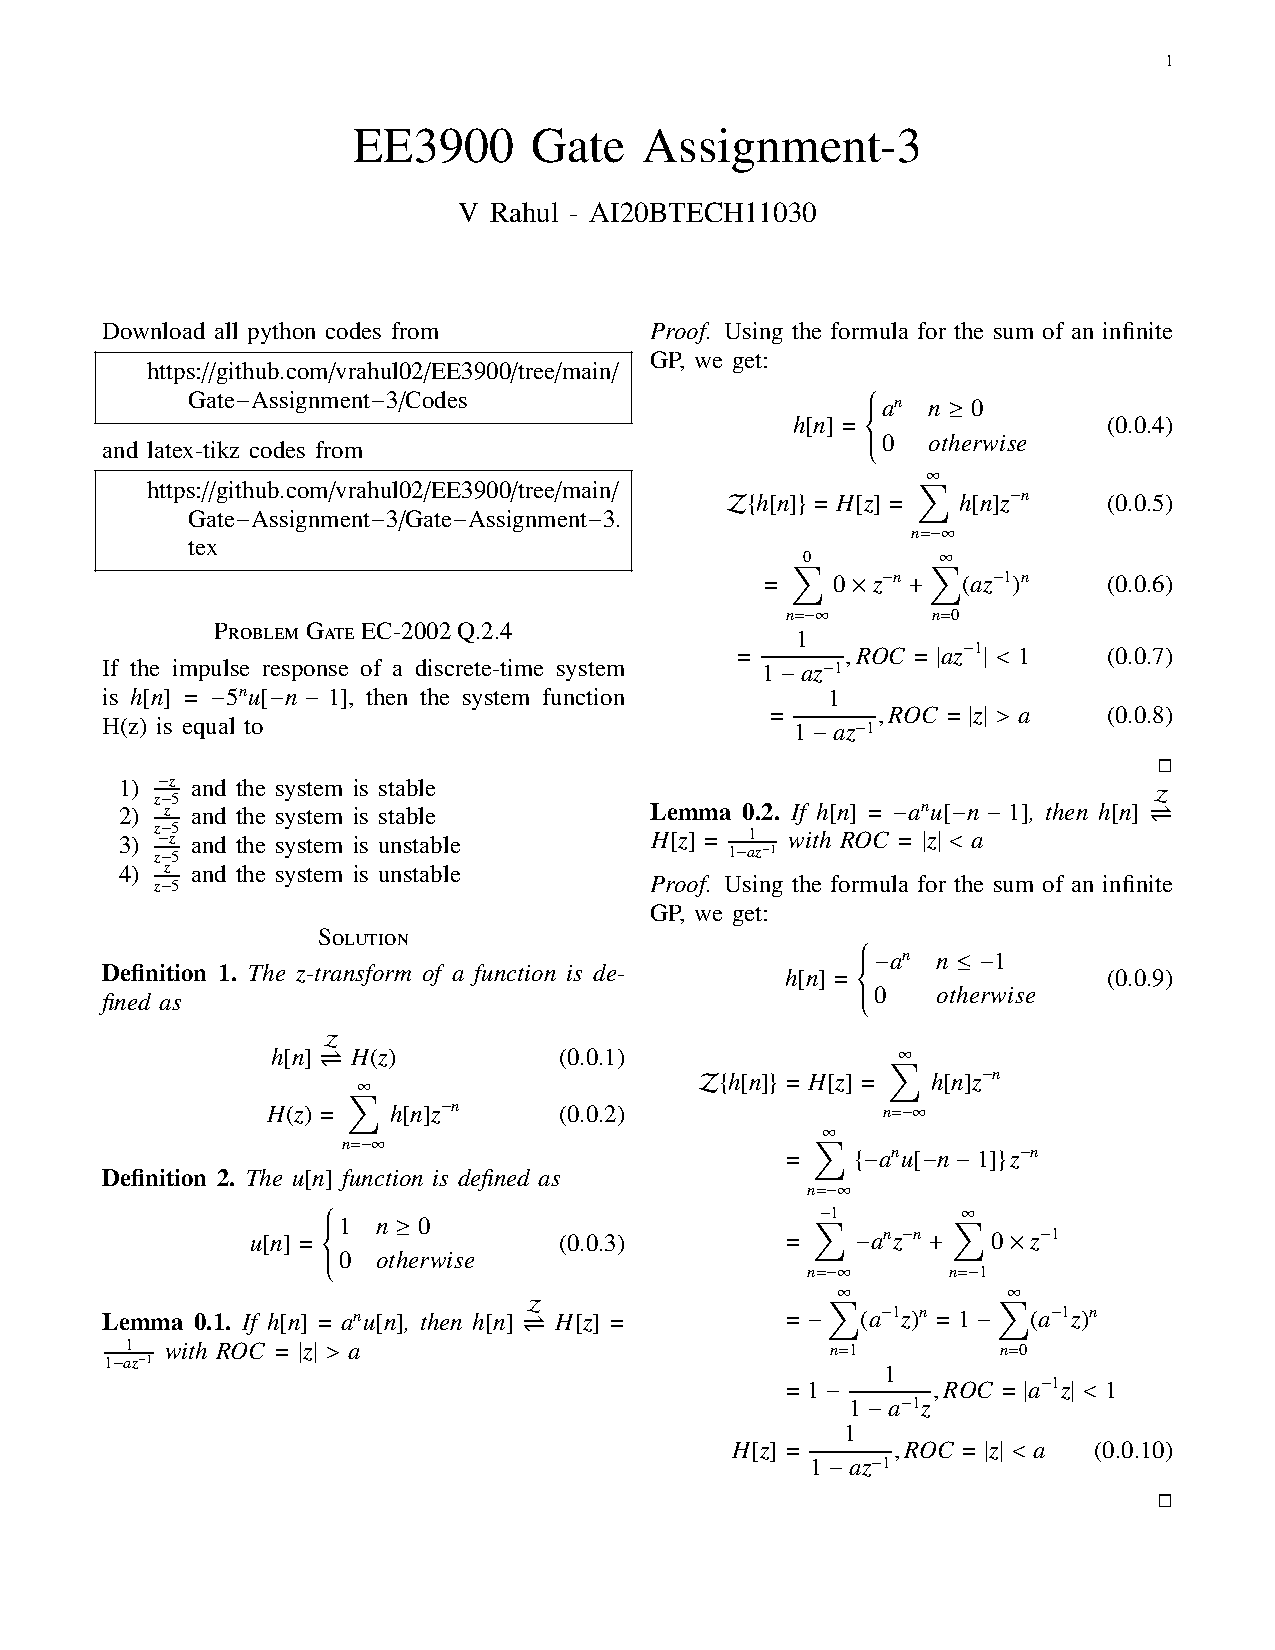
\includegraphics[width=\columnwidth]{Gate Assignment-3}
    \caption{Pole-zero plot of the system}
    \label{a}
\end{figure}\\
\begin{definition}\label{def:BIBO}
    An discrete-time system is BIBO stable if and only if its impulse response sequence $h[n]$ is absolutely summable, i.e,
    \begin{align}
        S=\sum_{n = -\infty}^\infty \abs{h[n]}<\infty
    \end{align}
\end{definition}
Using~\eqref{def:BIBO} and~\eqref{def:u_n}
\begin{align}
    S&=\sum_{n = -\infty}^\infty \abs{-5^nu[-n-1]}\\
     &= \sum_{n = -\infty}^{-1} {5^n} + \sum_{n = -1}^{\infty} 0\times {5^n}\\
    &=-\sum_{n = 1}^{\infty} 5^{-n}\\ 
    &=1-\sum_{n = 0}^{\infty} (5^{-1})^n
\end{align}
Using the formula for the sum of an infinite GP, we get:\\
\begin{align}
     S&= 1-\frac{1}{1 - 5^{-1}} \\
      &= \frac{-1}{4}<\infty
\end{align}
So for a bounded input we get bounded output. Thus it is a stable system.\\
Thus option 2) is correct
\end{document}